\documentclass[12pt]{ociamthesis}\usepackage[]{graphicx}\usepackage[]{color}
%% maxwidth is the original width if it is less than linewidth
%% otherwise use linewidth (to make sure the graphics do not exceed the margin)
\makeatletter
\def\maxwidth{ %
  \ifdim\Gin@nat@width>\linewidth
    \linewidth
  \else
    \Gin@nat@width
  \fi
}
\makeatother

\definecolor{fgcolor}{rgb}{0.345, 0.345, 0.345}
\newcommand{\hlnum}[1]{\textcolor[rgb]{0.686,0.059,0.569}{#1}}%
\newcommand{\hlstr}[1]{\textcolor[rgb]{0.192,0.494,0.8}{#1}}%
\newcommand{\hlcom}[1]{\textcolor[rgb]{0.678,0.584,0.686}{\textit{#1}}}%
\newcommand{\hlopt}[1]{\textcolor[rgb]{0,0,0}{#1}}%
\newcommand{\hlstd}[1]{\textcolor[rgb]{0.345,0.345,0.345}{#1}}%
\newcommand{\hlkwa}[1]{\textcolor[rgb]{0.161,0.373,0.58}{\textbf{#1}}}%
\newcommand{\hlkwb}[1]{\textcolor[rgb]{0.69,0.353,0.396}{#1}}%
\newcommand{\hlkwc}[1]{\textcolor[rgb]{0.333,0.667,0.333}{#1}}%
\newcommand{\hlkwd}[1]{\textcolor[rgb]{0.737,0.353,0.396}{\textbf{#1}}}%
\let\hlipl\hlkwb

\usepackage{framed}
\makeatletter
\newenvironment{kframe}{%
 \def\at@end@of@kframe{}%
 \ifinner\ifhmode%
  \def\at@end@of@kframe{\end{minipage}}%
  \begin{minipage}{\columnwidth}%
 \fi\fi%
 \def\FrameCommand##1{\hskip\@totalleftmargin \hskip-\fboxsep
 \colorbox{shadecolor}{##1}\hskip-\fboxsep
     % There is no \\@totalrightmargin, so:
     \hskip-\linewidth \hskip-\@totalleftmargin \hskip\columnwidth}%
 \MakeFramed {\advance\hsize-\width
   \@totalleftmargin\z@ \linewidth\hsize
   \@setminipage}}%
 {\par\unskip\endMakeFramed%
 \at@end@of@kframe}
\makeatother

\definecolor{shadecolor}{rgb}{.97, .97, .97}
\definecolor{messagecolor}{rgb}{0, 0, 0}
\definecolor{warningcolor}{rgb}{1, 0, 1}
\definecolor{errorcolor}{rgb}{1, 0, 0}
\newenvironment{knitrout}{}{} % an empty environment to be redefined in TeX

\usepackage{alltt}  % default square logo 
%\documentclass[12pt,beltcrest]{ociamthesis} % use old belt crest logo
%\documentclass[12pt,shieldcrest]{ociamthesis} % use older shield crest logo

%load any additional packages
\usepackage{amssymb}
\usepackage[english]{babel}
\usepackage{graphicx}
\usepackage{graphics}
\usepackage{adjustbox}
\usepackage{rotating}
\graphicspath{{figure/}}
\usepackage{amsmath}
\usepackage{dcolumn}
\usepackage{listings}
\usepackage{enumitem}
\newlist{todolist}{itemize}{2}
\setlist[todolist]{label=$\square$}
\usepackage{pifont}
\usepackage{url}
\usepackage{lipsum}
\usepackage{array}
\usepackage{float}
\usepackage[%
  backend=bibtex      % biber or bibtex
 ,style=numeric-comp    % Alphabeticalsch
 %,style=numeric-comp  % numerical-compressed
 ,sorting=none        % no sorting
 ,sortcites=true      % some other example options ...
 ,block=none
 ,indexing=false
 ,citereset=none
 ,isbn=true
 ,url=true
 ,doi=true            % prints doi
 ,natbib=true         % if you need natbib functions
]{biblatex}

\addbibresource{refs.bib} %Imports bibliography file

\newcommand{\cdifficile}{Clostridium \textit{difficile}}
\newcommand{\cdiff}{C. \textit{diff}}
\newcommand{\cmark}{\ding{51}}%
\newcommand{\xmark}{\ding{55}}%
\newcommand{\done}{\rlap{$\square$}{\raisebox{2pt}{\large\hspace{1pt}\cmark}}%
\hspace{-2.5pt}}
\newcommand{\wontfix}{\rlap{$\square$}{\large\hspace{1pt}\xmark}}
% Confidence interval
\newcommand{\ci}[3]{#1 (95\% CI, #2-#3)}
% Confidence interval with percent
\newcommand{\cip}[3]{#1\% (95\% CI, #2\%-#3\%)}

%input macros (i.e. write your own macros file called mymacros.tex 
%and uncomment the next line)
%\include{mymacros}

%note \\[1ex] is a line break in the title
\title{A Longitudinal Study of the Effect of Renal Failure on Readmission Rates of Patients with \textit{Clostridium Difficile}}

\author{Brian Detweiler}
\college{College of Arts and Sciences}  %your college

%\renewcommand{\submittedtext}{change the default text here if needed}
\degree{Master of Science}     %the degree
\degreedate{May 4, 2017}         %the degree date

%end the preamble and start the document
\IfFileExists{upquote.sty}{\usepackage{upquote}}{}
\begin{document}

%this baselineskip gives sufficient line spacing for an examiner to easily
%markup the thesis with comments
\baselineskip=18pt plus1pt

%set the number of sectioning levels that get number and appear in the contents
\setcounter{secnumdepth}{3}
\setcounter{tocdepth}{3}


\maketitle                  % create a title page from the preamble info

% include a dedication.Rnw file
%<<dedication, child='dedication.Rnw'>>=
%@
 
% include an acknowledgements.Rnw file%
%<<acknowledgements, child='acknowledgements.Rnw'>>=
%@

% include the abstract

\begin{abstract}
\cdifficile (\cdiff)
is a highly contagious endospore forming bacterium that is transferred
through physical contact with an infected surface. Symptoms range from diarrhea to
life-threatening colitis and is most commonly acquired in a hospital setting where
antimicrobials have been administered. Increased mortality in
\cdiff infected patients with renal failure comorbidities has appeared in the literature as early as 1998 \cite{Cunney1998}.
In this study, we analyze \cdiff trends from 2001-2014 using the \textit{National Inpatient Sample}. We also  
assess the risk of 30, 60, and 90 day readmissions in patients with comorbid \cdiff infection and renal failure conditions
using the \textit{Nationwide Readmissions Database} from 2010-2014. 
\end{abstract}

\begin{romanpages}          % start roman page numbering
\tableofcontents            % generate and include a table of contents
\listoffigures              % generate and include a list of figures
\listoftables
\end{romanpages}            % end roman page numbering


















%now include the files of latex for each of the chapters etc

\chapter{Introduction}

\section{Overview of \cdifficile}

\cdifficile, or \cdiff Infection (CDI) -
has been an increasing concern in the last two decades among healthcare providers. 
The organism itself is a resilient endospore-forming bacterium, resistant to heat, acid, and antibiotics,
and can survive on surfaces for up to 5 months, if proper sanitation is not carried out \cite{Gerding2008}.

In past years, the most common CDI cases occurred in elderly patients, 65 years or older,
who were admitted as inpatients in a hospital or nursing home setting, and given antimicrobial therapy.
In fact, it has become the most frequent nosocomial (hospital-acquired) disease, surpassing
methicillin-resistant Staphylococcus aureus (MRSA) \cite{Gupta2014}.

Antimicrobials deplete the healthy gut flora of the intestines which protect against harmful organisms like \cdiff \cite{Lamont2017}.

Adding to the complexity of the situation, \cdiff carriers can remain asymptomatic, making them stealth transporters
and allowing the disease to propagate undetected until it is too late. 

In 2013, the CDC estimated that around 250,000 Americans contracted CDI in a single year, causing 14,000 deaths.
That estimate was later updated to half a million in 2015, causing 15,000 deaths \cite{CDC2015, CDC2018}.
Another study puts that number even higher, at 29,000 deaths in 2011. 

CDI is also costly. The CDC estimates that in 2008, it cost acute healthcare facilities alone more than \$4.8 billion.
The mean cost of an incident of CDI was found to be \$11,498 (inflation adjusted to 2008 dollars)
and as high as \$15,397 when CDI was hospital acquired \cite{Dubberke2012}.


\section{Overview of Renal Failure}

While CDI is a singular diagnosis category, renal failure falls into one of two umbrella categories, acute kidney injury (AKI), 
and chronic kidney disease (CKD). AKI is further broken into subcategories. Acute tubular necrosis is the most common form of AKI.
Other subcategories include renal cortical necrosis, renal medullary necrosis, lesions, and a category for unspecified AKI. 

When evaluating the effect of renal failure on outcome variables, we first need to understand how renal failure is classified.

Chronic kidney disease is broken into categories based on stages that are calculated using one of the estimated Glomerular Filtration Rate
(GFR) equations. The equations model kidney health as a function of age, sex, race, and blood creatinine, a waste product that is produced from
normal muscle use. One of two formulas may be used, the Modification of Diet in Renal Disease (MDRD) formula \cite{Levey1999}, or the newer
Chronic Kidney Disease Epidemiology Collaboration (CKD-EPI) formula \cite{eGFR2018}. The models are included below to show the roles that
age, sex, and race play in the diagnosis of CKD.

\subsection{The MDRD and CKD-EPI Equations}

Patients are classified as having a particular CKD stage by testing their Glomerular Filtration Rate (GFR) using one of two equations.
Both equations measure the creatinine in a patient's blood with a serum creatinine test. Creatinine is a waste product produced by normal
muscle wear and tear. 

The MDRD equation encodes sex and race (African American or not) and does not rely on height or weight due to using the geneally accepted
mean surface area of the average adult, $1.73m^2$. GFR is expressed in units of mL/minute/$1.73m^2$.

\begin{equation} \label{mdrd}
\begin{split}
  GFR  &= 175 \times {S_{cr}}^{- 1.154} \times \text{Age}^{-0.203} \times 0.742 \cdot I(\text{F}) \times 1.212 \cdot I(\text{AA}) \\
\end{split}
\end{equation}

where:
\begin{itemize}
  \item F is female sex
  \item AA is African American race
  \item I is an indicator function that returns 1 if true, the reciprocal of the preceding term if false (thereby making the preceding term 1)
  \item $S_{cr}$ is serum creatinine in mg/dL
\end{itemize} 

The CKD Epidemiology (CKD-EPI) was a single equation selected out of a large number of candidate equations, that uses transformations of continuous
variables and additional variables and interactions. Serum creatinine is modeled as a 2-slope spline with sex-specific knots at 0.7 mg/dL for women 
and 0.9 mg/dL for men. It was shown to outperform the MDRD, with lower bias and increased precision.  \cite{Levey2009, eGFR2018}

\begin{equation} \label{ckdepi}
\begin{split}
  GFR &= 141 \times min\bigg(\frac{S_{cr}}{\kappa}, 1\bigg)^{\alpha} \times max\bigg(\frac{S_{cr}}{\kappa}, 1\bigg)^{-1.209} \\
      &\times 0.993^{\text{Age}} \times 1.018 \cdot \text{I}(\text{F}) \times 1.159 \cdot \text{I}(\text{AA}) \\
\end{split}
\end{equation}

where:
\begin{itemize}
  \item $\kappa$ is 0.7 for females and 0.9 for males
  \item $\alpha$ is -0.329 for females and -0.411 for males
\end{itemize} 

\subsection{Classifying Chronic Kidney Disease}

Once the GFR is calculated using either the MDRD or the CKD-EPI formulas, 
patients can be placed into one of five categories. Table \ref{tab:gfr} shows the 
GFR rating along with the stage of CKD and the level of kidney function. \textbf{585} is used in the ICD-9-CM coding system
to indicate CKD. If the level is known, a more specific coding is used. \textbf{585.1-585.5} indicate CKD Stage 1 through 5.
\textbf{585.6} is used for end stage renal disease (dialysis or transplant), and \textbf{585.9} is used if the level is unspecified.

\begin{table}[]
\centering
\label{my-label}
\begin{tabular}{lllll}
CKD Stage & Description             & GFR        & Kidney Function & ICD-9-CM \\
\hline
1         & Normal function         & 90+        & 90-100\%        & 585.1    \\
2         & Mild loss               & 60-89      & 60-89\%         & 585.2    \\
3         & Mild to severe          & 30-59      & 30-59\%         & 585.3    \\
4         & Severe                  & 15-29      & 15-29\%         & 585.4    \\
5         & Kidney failure          & 15 or less & 15\% or less    & 585.5    \\
\end{tabular}\caption{GFR classifications for stages of Chronic Kidney Disease}\label{tab:gfr}
\end{table}

\subsection{End stage renal disease}

When CKD reaches Stage 5, it is considered end stage renal disease (ESRD). Dialysis or a kidney transplant is needed to stay alive.
The most common causes of ESRD are diabetes and high blood pressure. Risk of ESRD also increases with age. 


\section{Index Admissions and Readmissions}

An inpatient admission begins on the first day a patient is admitted to a hospital under a doctor's order. The 
last day before discharge is the last inpatient day \cite{Medicare}.

Readmissions are subsequent admissions from a given \textit{index} admission within a specified time interval.
Methods and inclusion/exclusion criteria for determining an index admission and readmissions vary. 

\subsection{Readmissions and the ACA}

A 2014 study done by the Agency for Healthcare Research and Quality (AHRQ) under the Healthcare Cost and Utilization
Project (HCUP) found hospital readmissions accounted for about \$41.3 billion in hospital costs \cite{Hines2014}.

Under the Readmission Reduction Program, a provision of the Affordable Care Act, 
Hospitals face penalties on Medicare payments if they exceed certain 30-day readmission standards. While the 
American Hospital Association strongly opposes the measure, citing a lack of control over the chain of events
that can lead to readmission \cite{Rice2015, AHA2018}, the Affordable Care Act is still the rule of law, and hospitals must seek
to reduce readmissions in order to avoid penalties.

For this reason, readmission statistics are an important key metric for hospitals interested in optimizing 
their operations. Using large surveys, researchers are able to determine trends and end results, but not necessarily 
causes, of readmissions. Still, high level trends can point healthcare providers in a direction where they can
more efficiently focus their attention. Studies like this one focus on narrow cases where a better understanding can 
contribute to reduced readmissions and an overall reduction in penalties.

\subsection{Readmission measures}

The Centers for Medicare \& Medicaid Services (CMS) sets guidelines that hospitals must follow to avoid penalization on Medicare payments. 
The CMS measures "excess readmissions" as a ratio of predicted-to-expected readmissions and each hospital's relative performance, based on
a 30-day risk standardized measure. All-cause unplanned readmissions to the same or another applicable acute care hospital, 
occurring within 30 days - for any reason, regardless of principal diagnosis - from the index admission are counted in this measure.
Some planned readmissions are not counted \cite{HRRP}. 

For fiscal years 2013 to 2018, the following formula is used to calculate the Payment Readjustment Factor (PRF):

\begin{equation} \label{prf}
\begin{split}
  \text{PRF} &= 1 - min\bigg(0.03, \sum_{dx} \frac{\text{Payment}(dx) \cdot max\big((\text{ERR}(dx) - 1.0), 0\big)}{\text{All payments}}\bigg) \\
\end{split}
\end{equation}
 
Where $dx$ is one of six measure cohorts: 

\begin{itemize}
  \item acute myocardial infarction (AMI)
  \item heart failure (HF)
  \item pneumonia
  \item chronic obstructive pulmonary disease (COPD)
  \item coronary artery bypass graft (CABG) surgeries
  \item elective primary total hip and/or total knee arthroplasty (THA/TKA)
\end{itemize}

ERR is a hospital's ratio of predicted-to-expected readmissions against $dx$, and payment refers to base operating DRG payments.
An ERR greater than 1.0 indicates that a hospital performed worse than the average performance of all hospitals. \cite{HRRPPaymentAdjustment, Lessa2015}.


\section{Overview of the data}

The data obtained for this study comes from the Agency for Healthcare Research and Quality (AHRQ),
under the Department of Health and Human Services (DHHS). ARHQ sponsors the
Healthcare Cost and Utilization Project (HCUP), a collection of databases including the Nationwide Inpatient Sample (NIS) and
the Nationwide Readmissions Database (NRD) \cite{HCUPOverview}. For this study, we obtained years 2001-2014 of the NIS, and
2010-2014 of the NRD.

Both datasets are based on complex survey designs. The Primary Sampling Units (PSUs) are hospitals, stratified by region,
teaching status, and bedsize. Weights are calculated for each discharge which are used to "map" the sample back to an unbiased
representation of the survey population \cite{Heeringa2017}.

\subsection{The Nationwide Inpatient Sample (NIS)}

The Agency for Healthcare Research (AHRQ) has been conducting the National (later renamed to "Nationwide") Inpatient
Sample since 1988, as part of the Healthcare Cost and Utilization Project (HCUP). It estimates a weighted 35 million
hospitalizations per calendar year using around 7-8 million unweighted discharges per year. It is the largest database
of its kind in the United States \cite{NISOverview}.

\subsection{The Nationwide Readmissions Database (NRD)}

Similar to the NIS, the NRD tracks hospitalizations. In addition, it tracks patients across admissions, using an ID key,
an admission reference date, and a length of stay for each admission. This allows analysts to track anonymized readmission cases.
The NRD tracks around 14 million unweighted patients, when weighted, estimates about 36 million weighted patients across admissions 
per calendar year \cite{NRDOverview}.

\subsection{Limitations}

Working on such a rich dataset does not come without limits. Prior to obtaining the NIS or NRD, analysts must take the HCUP
Data Usage Agreement (DUA). At a high level, HCUP requires that researchers protect individual identities. Cell sizes (groups of people)
where $n \le 10$ may not be reported. Attempting to identify individual patients or health care providers through vulnerability or penetration testing, 
or any other means, is prohibited. For instance, if an analyst noticed that a certain hospital used a particular coding scheme that was unique 
to that hospital and could be used to identify aspects of a patient, the analyst may not use this information. Furthermore, probing for such
vulnerabilities is prohibited as well. Publication of any methodology that could identify individuals is prohibited.

Furthermore, HCUP data may only be used for research, not for commercial or competitive purposes. Institutions may not be contacted
to verify any of the data within the HCUP datasets either. 

For the above reasons, the data may also not be posted online, and anyone wishing to work with or even see the data must take the DUA class and
sign the agreement \cite{HCUPDUA}.

In a couple of recent publications, Khera and Krumholz expanded on these base requirements and offered a checklist \cite{Krumholz2017} 
for analysts to follow as they work with the NIS. In a followup study, they found only 10.5\% (95\% CI, 4.7\%-16.4\%) of published research
projects based on NIS data followed all of the guidelines \cite{Khera2017}.

Listed below are the guidelines from Khera and Krumholz, and notes on how we have conformed to them.


\begin{itemize}
  \item  \textbf{Section A: Research Design}
  \begin{todolist}
  \item[\done] Does the study consider that it can only detect disease conditions, procedures, and diagnostic tests in hospital settings?
  
  \textbf{Yes, we make no assumptions about events occurring outside of the hospital setting.}
  
  \item[\done] Does the study acknowledge that it includes encounters, not individual patients?
  
  \textbf{Yes, all of our assumptions are made upon the basis of inpatient discharges and readmissions, not individuals.}
  
  \item[\done] Does the study avoid diagnosis/procedure-specific volume assessments for units that are not part of the
  sampling frame of the NIS, and are therefore not representatively sampled, including
  
  \begin{itemize}
    \item geographic units, like U.S. states
    \item healthcare facilities (after 2011)
    \item individual healthcare providers?
  \end{itemize} 
          
  \textbf{Yes, we only make assessments at the national level.}
  
  \end{todolist}
  
  \item  \textbf{Section B: Data Interpretation}
  \begin{todolist}
  \item[\done] Does the study attempt to identify disease conditions or procedures of interest using administrative 
  codes or their combinations that have been previously validated?
 
  \textbf{Yes, when checking for renal failure, the comorbidity indicators (\texttt{renlfail, cm\_renlfail}) were used 
  before assessing ICD-9-CM codes.}
  
  \item[\done] Does the study limit its assessments to only in-hospital outcomes, rather than those occurring after discharge?
  
  \textbf{Yes, the only outcome assessments were readmission status and mortality (\texttt{died}), both of which are in-hospital events.}
  
  \item[\done] Does the study distinguish complications from comorbidities or clearly note where it cannot?
  
  \textbf{Yes, renal failure comorbidities were distinguished using the the comorbidity indicators (\texttt{renlfail, cm\_renlfail}). 
  CDI while most often a complication, cannot usually be distinguished between complication and comorbidity however.}
  
  
  \end{todolist}
  
  \item  \textbf{Section C: Data Analysis}
  \begin{todolist}
  \item[\done] Does the study clearly account for the survey design of the NIS and its components -clustering, stratification, and weighting?
 
  \textbf{Yes, the R \texttt{survey} package was used to account for survey design.}
  
  \item[\done] Does the study adequately address changes in data structure over time (for trend analyses)?
  
  \textbf{Yes, since we are only doing national-level assessments, and we are not using ICD-10-CM codes in the 2015 datasets, 
  we don't need to worry about the changes in the survey design.}
  
  \end{todolist}
  
\end{itemize}

\subsection{Goals}

The goals of this study are to evaluate trends in CDI and renal failure over the period of 2001-2014 using the NIS, and 
to determine risk factors of readmission for CDI patients over the period of 2010-2014 using the NRD.

\chapter{Methods}




All analyses were done in R version 3.4.3 (2017-11-30) on an x86\_64-pc-linux-gnu (64-bit) 
running Ubuntu 16.04.4 LTS. 
Complex survey designs of the NIS and NRD  were accounted for using the \texttt{survey} package, version 
3.33-2 \cite{Lumley2018}. Data were stored and retrieved in
MonetDB using MonetDBLite version 0.5.1 \cite{Muehleisen2018}.

\section{Data source}

Years 2001-2014 of the NIS, as well as years 2010-2014 of the NRD were provided courtesy of Creighton University
School of Medicine. Both datasets originate in comma-separated variables (CSV) format. 

The NIS covers between 7-8 million unweighted patients per calendar year, resulting in file sizes around 3 GB on average,
totaling around 43 GB of raw ASCII text.

\begin{lstlisting}[language=Bash,caption={Showing file sizes for the NIS dataset from 2001-2014},captionpos=b]
  $ l -ha NIS* | awk '{print $5, $9}'
  2.7G NIS2001.csv                                                          
  2.9G NIS2002.csv                                                          
  3.0G NIS2003.csv                                                          
  3.1G NIS2004.csv                                                          
  3.1G NIS2005.csv                                                          
  3.1G NIS2006.csv                                                          
  3.4G NIS2007.csv                                                          
  3.4G NIS2008.csv                                                          
  3.5G NIS2009.csv
  3.6G NIS2010.csv
  3.7G NIS2011.csv
  2.6G NIS2012.csv
  2.6G NIS2013.csv
  2.8G NIS2014.csv
\end{lstlisting}

The NRD is normalized into 4 different files, 3 discharge-level files and a hospital-level file.

The \texttt{Core} file contains data elements necessary for readmission analysis. The \texttt{Severity} files
contain data related to the severity of the patients' conditions, including, for our purposes, comorbidity flags.
The \texttt{DX\_PR} file (diagnoses and procedures) file contains ICD-9-CM codes and other fields related to
diagnoses and procedures. Finally, the hospital file contains information on the hospital characteristics.

The NRD is a record of around 14 million unweighted admissions per calendar year with identifiers that allow analysts 
to track readmissions from a particular index event.

\begin{lstlisting}[language=Bash,caption={Showing file sizes for the NRD dataset from 2010-2014},captionpos=b]
  $ l -ha NRD*/*.CSV | awk '{print $5, $9}' | sed -e 's/ /\t/'
  5.0G    NRD2010/NRD_2010_Core_V2.CSV
  3.4G    NRD2010/NRD_2010_DX_PR_GRPS_V2.CSV
  88K     NRD2010/NRD_2010_Hospital_V2.CSV
  1.2G    NRD2010/NRD_2010_Severity_V2.CSV
  5.1G    NRD2011/NRD_2011_Core_V2.CSV
  3.4G    NRD2011/NRD_2011_DX_PR_GRPS_V2.CSV
  87K     NRD2011/NRD_2011_Hospital_V2.CSV
  1.2G    NRD2011/NRD_2011_Severity_V2.CSV
  4.9G    NRD2012/NRD_2012_Core_V2.CSV
  3.3G    NRD2012/NRD_2012_DX_PR_GRPS_V2.CSV
  82K     NRD2012/NRD_2012_Hospital_V2.CSV
  1.1G    NRD2012/NRD_2012_Severity_V2.CSV
  5.2G    NRD2013/NRD_2013_Core.CSV
  3.4G    NRD2013/NRD_2013_DX_PR_GRPS.CSV
  92K     NRD2013/NRD_2013_Hospital.CSV
  1.1G    NRD2013/NRD_2013_Severity.CSV
  6.6G    NRD2014/NRD_2014_Core.CSV
  4.1G    NRD2014/NRD_2014_DX_PR_GRPS.CSV
  98K     NRD2014/NRD_2014_Hospital.CSV
  1.2G    NRD2014/NRD_2014_Severity.CSV
\end{lstlisting}

This totals to over 50 GB of raw ASCII text. 

\subsection{Persistence}

There are numerous ways to handle a dataset of this size. If we know exactly what unique codes we want,
we could simply \texttt{grep} for them. However, this isn't scalable and we would not be able to calculate
population proportions.

For this project, we imported the data into MonetDBLite, an in-process version of MonetDB. 
We chose MonetDB, because it fits well in the academic space, being open source with strong R 
integration and good community support.
It also fits well in the data warehousing space, being a pioneer in column-store technologies. 

Column-store databases partition each column as an array, making data retrieval extremely fast when
only a subset of the columns need to be loaded into memory \cite{MonetDB}.

\subsection{Diagnosis and procedure codes}

The International Classification of Diseases, Ninth Revision, Clinical Modification (ICD-9-CM) is based on the World Health Organization's Ninth Revision,
International Classification of Diseases (ICD-9). It is the coding standard for diseases and procedures used in the NIS and NRD up to October, 2015, when
HCUP upgraded to ICD-10-CM. 

Although we had access to the 2015 NRD data, it was not used due to the added complexity of accounting for ICD-10-CM changes, as well as not having 2015
data for NIS, which would have caused inconsistencies in trend analysis. 

With the acknowledgement that ICD-9-CM codes are not perfect \cite{Uchiyama2015}, they are still the best thing we have for longitudinal 
epidemiological studies on a large scale. The ICD-9-CM diagnosis codes are stored in  fields \texttt{dx1, dx2,} $\hdots$ \texttt{dx30}.
\texttt{dx1} is the principal diagnosis, or the diagnosis primarily responsible for the patient being admitted. This is not always clear cut,
as patients often have multiple diseases, and any one could be responsible for their admission, so in these cases, they are often
coded with consideration to cost and reimbursement. 

These were queried for code \textbf{00845} (\textit{Intestinal infection due to Clostridium difficile}). 
The decision not to look exclusively at \texttt{dx1}, the principal diagnosis, was deliberate, due to the nature of CDI. Patients rarely contract CDI
independently. It is typically contracted while in a hospital setting while being treated for a separate disease. 

To complicate matters, ICD-9-CM codings are not an exact science, and are often done based on cost and seriousness of comorbid conditions. Coders must use
their judgement for determining a principal diagnosis when comorbid conditions are present \cite{Avery2011}. For this reason, we simply queried for
the presence of the condition on any diagnosis field. 

The same was done for renal failure codes, shown in table \ref{icd9renal}. 

\begin{table}[]
\centering
\begin{tabular}{ll}
ICD-9-CM Code  & Description          \\
\hline
584   & Acute kidney failure \\
584.5 &	Acute kidney failure with lesion of tubular necrosis convert \\
584.6 &	Acute kidney failure with lesion of renal cortical necrosis convert \\
584.7 &	Acute kidney failure with lesion of renal medullary [papillary] necrosis \\
584.8 &	Acute kidney failure with lesion of with other specified pathological lesion in kidney \\
584.9 &	Acute kidney failure, unspecified \\
585   & Chronic kidney disease (ckd) \\
585.1 &	Chronic kidney disease, Stage I \\
585.2 &	Chronic kidney disease, Stage II (mild) \\
585.3 &	Chronic kidney disease, Stage III (moderate) \\
585.4 &	Chronic kidney disease, Stage IV (severe) \\
585.5 &	Chronic kidney disease, Stage V (end stage) \\
585.6 &	End stage renal disease \\
585.9 &	Chronic kidney disease, unspecified \\
586   &	Renal failure, unspecified \\
\end{tabular}
\caption{ICD-9-CM renal failure codes}
\label{icd9renal}
\end{table}

For trend analysis, the CDI and renal failure selections were joined. This provided full samples of
CDI and renal patients, as well as patients with both.


\subsection{Determining index admissions and readmissions}

Unlike the NIS, the NRD allows tracking patients across hospital visits within a given calendar year.
The field \texttt{nrd\_visitlink} provides a key that identifies a single patient across multiple visits.
To determine temporality, a length of stay field (\texttt{los}) is provided for each visit, as well as
a reference date, \texttt{nrd\_daystoevent}. To ensure anonymity, a randomly selected date is chosen for 
each patient. \texttt{nrd\_daystoevent} then references the random date and lists the days from the epoch date.
This way, no precise date can be determined, thereby protecting patient privacy, while providing the researcher
with the data he or she needs. 

The NRD leaves readmission determination up to the analyst. First an index event must be chosen. 
We selected all cases of CDI (ICD-9-CM code \textbf{00845}) and retrieved all unique \texttt{nrd\_visitlink}
identifiers. Then a second query was performed retrieving all events for the \texttt{nrd\_visitlink} identifiers.


We then grouped the cases first by \texttt{nrd\_visitlink}, then chronologically. Then, we scanned for the first
occurrence of a CDI event (ICDM-9-CM code \textbf{00845}) and marked it as the index event. All information from
the index event was stored in a "patient profile" object. The remaining patient admissions, if any, were scanned.
If the event contained a CDI identifier and fell within the given readmission day window (30, 60, and 90 days, separately),
the event was considered a readmission and the number of readmissions were stored. If the patient died on a readmission,
that was also stored. If the secondary event fell outside of the readmission window, it was considered another index event, 
and the process started over. The state diagram is shown in Figure \ref{fig:readmission-state-diagram}.

\begin{figure}[h]
\centering
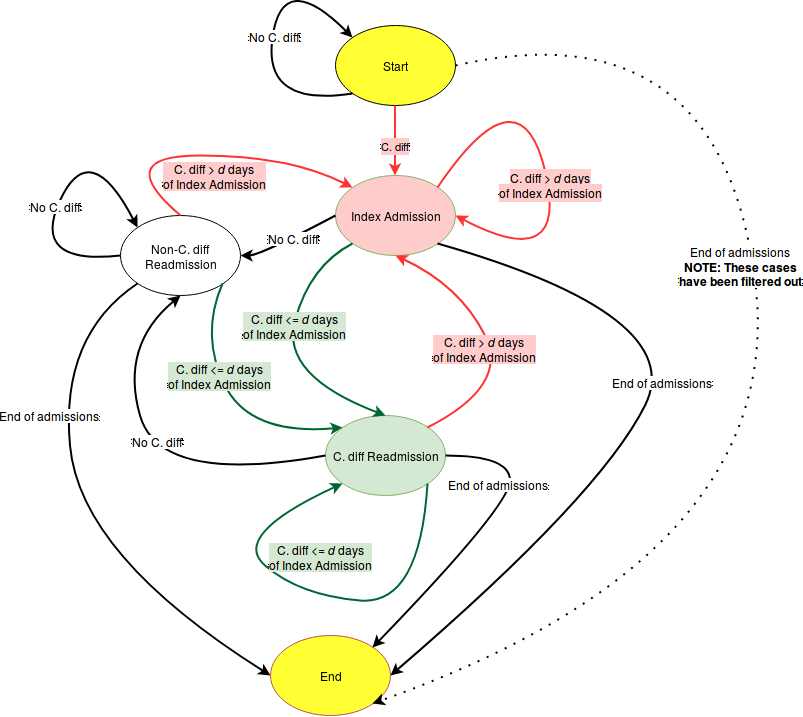
\includegraphics[scale=0.5]{readmission-state-diagram.png} 
\caption{State diagram for determining what constitutes an index admission and a subsequent readmission.
Additional rules include cutting off index events by October, November, or December, depending on whether we are looking for 90, 60, 30 day readmissions, respectively;
filtering out deaths on index events;
lengths of stay that included transfers and same-day stays;
and infants less than 1 year of age, where \cdiff bacteria are common but the patient shows no symptoms.}
\label{fig:readmission-state-diagram} 
\end{figure}
The following additional rules were applied for determining index events for \textit{d}-day readmissons, where $d \in \{30, 60, 90\}$:

\begin{enumerate}
    \item For years 2010-2014: ($1 \le \text{DMONTH} \le 12 - ceil(d/30)$)
    
    We needed to cut off index events with enough time to determine if there was a readmission, since only calendar years can be analyzed.
    
    \item $\text{DIED} \ne 0$
    
    A death on index does not allow for readmission.
    
    \item $\text{LOS} > 0$
    
    A length of stay equal to zero represents transfers and same-day stays that were combined which represents a more complex type of care \cite{NRDIntroduction2013}.
    
    \item $AGE > 0$
  
    About 70\% of infants under one year of age carry \cdiff without showing signs or symptoms of infection \cite{Lamont2017}. 
    
\end{enumerate}




\subsection{Choosing features}

To determine renal failure comorbidities, the \texttt{cm\_renlfail} flag was first used, and then more specific ICD-9-CM codes were identified. Acute kidney failure, 
or acute kidney injury (AKI) were grouped by all sub-category codes into a single AKI category. This included codes \textbf{584}, \textbf{584.5}, \textbf{584.6}, \textbf{584.7}, 
\textbf{584.8}, and \textbf{584.9} (see Table \ref{icd9renal}).

Chronic kidney disease (CKD) stages were individually analyzed, but unspecified or unknown CKD cases were grouped, (ICD-9-CM codes \textbf{585} and \textbf{585.9}). 

Additionally, we considered hospital characteristics as independent factors, including hospital control (Government, nonfederal; Private, non-profit; Private, invest-own), 
urban/rural designation (9 categories from smallest to largest), teaching designation, and bedsize. 

Hospital urban/rural designations contained 9 categories 1 being the largest and 9 being the smallest. These were reversed in order to have a meaningful effect in the regression.

Sex was also included in the regression.

Patients' age is included in the eGFR formula, and as such, would be a confounding variable, so it was not included in the regression.

\section{Statistical analysis}

Descriptive and inferential statistics were done using the NIS and NRD complex survey design, 
supplying \texttt{hospid} as the clusters, \texttt{nis\_stratum} as the strata, and \texttt{discwt} as the weighting. 
Lonely primary sampling units (PSU) - in our case, hospitals - were excluded using \texttt{options(survey.lonely.psu="remove")} \cite{LonelyPSUs}.

The primary readmission analysis was done with multivariable logistic regression to determine the effect of the covariates and confounding variables
on the likelihood of being readmitted with CDI under the three readmission windows, 30, 60, and 90 days. Logistic regression is used throughout
the medical literature to explain effects on a binary outcome variable. At its core is a linear model that is both effective and easy to explain. 

The odds are given by

\begin{equation} \label{logistic}
    Pr(\text{readmitted}) = \frac{e^{\beta \mathbf{X}}}{1 - e^{\beta \mathbf{X}}}
\end{equation}

where $\mathbf{X}$ is a matrix consisting of a constant (slope), and the feature variables shown in Table \ref{logistic-regression-features}.
The full list of regression coefficient estimates are provided in Appendix A
(Tables \ref{30-day-readmission-fit}, \ref{60-day-readmission-fit}, and \ref{90-day-readmission-fit}).


Note the following:

\begin{itemize}
  \item \texttt{hosp\_hcontrl\_govt} and \texttt{hosp\_hcontrl\_priv\_np} were compared against a baseline of 
        \texttt{hosp\_hcontrl\_priv\_invest\_own}, which represents a hospital's control/ownership of private, investor owned (proprietary)
  \item \texttt{hosp\_urcat4} is a discrete variable from 1 to 4, representing the smallest to largest areas. In this case, an increasing integer
        size corresponds to an increasing metropolitan area size. The original variable used a descending order, where 1 was the largest and 4 was the
        smallest, so we reversed the order to make the variable naturally meaningful without the need for dummy variables
  \item \texttt{hosp\_ur\_teach\_metro} and \texttt{hosp\_ur\_teach\_metro\_teaching} were compared against a baseline of \texttt{hosp\_ur\_nonmetro}, 
        which did not distinguish between teaching and non-teaching because rural hospitals  were rare 
  \item \texttt{hosp\_bedsize} is a discrete variable from 1 to 3, indicating small, medium, and large hospital bedsizes
  \item \texttt{female} is a binary variable, 0 is male, 1 is female
  \item \texttt{acute\_kidney\_failure} grouped all forms of AKI. The baseline is not having any form of AKI
  \item \texttt{chronic\_kidney\_disease2-6} and \texttt{chronic\_kidney\_disease\_unk} are the various stages of CKD, compared against a baseline of CKD Stage 1 (mostly healthy)
  \item \texttt{renal\_failure\_unspecified} was compared against not having any unspecified renal failure
\end{itemize}

\begin{table}[]
\centering
\begin{tabular}{ll}
  NRD variable   & Description \\
\hline
  hosp\_hcontrl\_govt            & Hospital's ownership/control - Government, nonfederal  \\
  hosp\_hcontrl\_priv\_np         & Hospital's ownership/control - Private, not-profit  \\ \\
  %hosp\_hcontrl\_priv\_invest\_own & NO & YES & Hospital's ownership/control category - Private, invest-own  \\ \\
  hosp\_urcat4                  & Urban-rural categorization (1-4, smallest to largest) \\
  %hosp\_ur\_nonmetro & NO & YES & Hospital teaching status - non-metro \\
  hosp\_ur\_teach\_metro          & Hospital teaching status - metro, non-teaching  \\
  hosp\_ur\_teach\_metro\_teaching & Hospital teaching status - metro, teaching \\
  hosp\_bedsize                 & Hospital bedsize (1-3, small to large)\\
  %male    & NO & YES & Sex, male \\
  female                       & Sex, binary, female \\
  acute\_kidney\_failure         & AKI, all types \\
  chronic\_kidney\_disease2      & CKD Stage 2 \\
  chronic\_kidney\_disease3      & CKD Stage 3 \\
  chronic\_kidney\_disease4      & CKD Stage 4 \\
  chronic\_kidney\_disease5      & CKD Stage 5 \\
  chronic\_kidney\_disease6      & ESRD \\
  chronic\_kidney\_disease\_unk  & CKD, unknown \\
  renal\_failure\_unspecified    & Renal failure, unspecified \\
\end{tabular}
\caption{ICD-9-CM renal failure codes}
\label{logistic-regression-features}
\end{table}

Age was not included, because it is factored in to the CKD stage classification in the GFR equations, \ref{mdrd} and \ref{ckdepi}.

The model was fitted independently on each year's data. 
Another approach would be to include the years as independent variables and attempt to fit the entire dataset. Because the dataset is very large,
a single all-year fit was somewhat impractical due to hardware resource limitations. From a practical aspect, we are able to capture more nuance in modeling individual
years, given each year is a separate independent data set, and medical trends do change over time. Fitting 5 years of data all at once is likely to miss smaller subtleties, 
such as increases or decreases in particular coefficient estimates over time. 

Variance estimation was done using the non-parametric method of Jackknife Repeated Replication (JRR), 
specifically the JKn approach, which is the default in the \texttt{survey} package. Details on JKn and other approaches
to variance estimation can be found in \cite{Heeringa2017}.
Replication methods have shown better precision and reduced bias compared to Taylor Series Linearization \cite{Chowdhury2013, Smith2000}. 

All charts were done with the \texttt{ggplot2} package \cite{Wickham2016}, and the coefficient tables in Appendix A were done with the \texttt{stargazer} package \cite{Hlavac2018}. 

All code for this project can be found on the author's GitHub account at \cite{Detweiler2018}. A journal has also been kept, documenting the research process, which can
be found on the author's website at \cite{DetweilerWebsite2018}.

\chapter{Results}


\section{Trends}

\begin{knitrout}
\definecolor{shadecolor}{rgb}{0.969, 0.969, 0.969}\color{fgcolor}\begin{figure}

{\centering \includegraphics[width=\maxwidth]{figure/disease_trends_cdi-1} 

}

\caption[CDI trends show a somewhat linearly increasing trend]{CDI trends show a somewhat linearly increasing trend. If we extrapolate to 2018, we have a rough idea of the proportion of the inpatient population we can expect to be diagnosed with CDI.}\label{fig:disease_trends_cdi}
\end{figure}


\end{knitrout}
\label{fig:disease_trends_cdi}

\begin{knitrout}
\definecolor{shadecolor}{rgb}{0.969, 0.969, 0.969}\color{fgcolor}\begin{figure}

{\centering \includegraphics[width=\maxwidth]{figure/age_distribution_over_time-1} 

}

\caption[CDI is trending into younger generations in recent years]{CDI is trending into younger generations in recent years.}\label{fig:age_distribution_over_time}
\end{figure}


\end{knitrout}
\label{fig:age_distribution_over_time}

\begin{knitrout}
\definecolor{shadecolor}{rgb}{0.969, 0.969, 0.969}\color{fgcolor}\begin{figure}

{\centering \includegraphics[width=\maxwidth]{figure/cdi_kurtosis_trends-1} 

}

\caption[The age distrubution of CDI is becoming more platykurtic and less left-skewed, indicating that the CDI is starting to infect younger people in recent years]{The age distrubution of CDI is becoming more platykurtic and less left-skewed, indicating that the CDI is starting to infect younger people in recent years. }\label{fig:cdi_kurtosis_trends}
\end{figure}


\end{knitrout}
\label{fig:cdi_kurtosis_trends}

\begin{knitrout}
\definecolor{shadecolor}{rgb}{0.969, 0.969, 0.969}\color{fgcolor}\begin{figure}

{\centering \includegraphics[width=\maxwidth]{figure/age_quantile_trends-1} 

}

\caption[The median age for inpatient CDI admissions has been sharply declined since 2006]{The median age for inpatient CDI admissions has been sharply declined since 2006. The vertical bars indicate a 95\% confidence interaval.}\label{fig:age_quantile_trends}
\end{figure}


\end{knitrout}

\label{fig:age_quantile_trends}



Over the 14 year period, from 2010 - 2014, the proportion of inpatients with CDI increased from 
\cip{0.003998292}{0.003773284}{0.004236661} in 2001, roughly 
\ci{141,540}{133,574}{149,978} cases, to
\cip{0.01023635}{0.01004522}{0.01043108} in 2014, or
\ci{362,367}{355,601}{369,260} cases - 
a difference of about 0.006238055\%, or 220,827 people. 

In Figures \ref{fig:disease_trends_cdi} and \ref{fig:age_distribution_over_time}, we can see the median age for inpatient CDI has been lowering over the years.
In fact, the entire distribution of CDI cases by age is becoming less left-skewed and more mesokurtic indicating a trend toward a more normal distribution 
(Figure \ref{fig:cdi_kurtosis_trends}). 

Figure \ref{fig:age_quantile_trends} shows the median age of CDI lowering from 73 years old in the mid-2000s, to about 68 years old in 2014. The ESRD distribution
over age (shown in Figure \ref{fig:disease_trends_esrd}) does not seem to have changed much since the ICD-9-CM 
coding standards were changed in 2005 to require more specific identifiers for renal failure patients.

Renal failure patients as a whole have become a very significant proportion of the inpatient population, far outpacing CDI, as shown in Figure \ref{fig:disease_trends_cdi_renal}.


We can also separate the trends over time by age groups, broken down into 5-year buckets. Figure \ref{fig:cdi_age_ts} shows more interesting trends.
Notably, nearly every age group is increasing in the number of CDI cases, except the 75-90 year groups, which appear to be on something of a downward trend.
The 50-75 year group are showing steady increases and are poised to take the lead on the number of CDI occurrences. 


\begin{knitrout}
\definecolor{shadecolor}{rgb}{0.969, 0.969, 0.969}\color{fgcolor}\begin{figure}

{\centering \includegraphics[width=\maxwidth]{figure/disease_trends_cdi_renal-1} 

}

\caption[Comparitively, CDI occurrences are not increasing as rapidly as renal diseases]{Comparitively, CDI occurrences are not increasing as rapidly as renal diseases. The sharp spikes from 2004-2006 were likely due to ICD-9-CM coding requirements implemented in October of 2005.}\label{fig:disease_trends_cdi_renal}
\end{figure}


\end{knitrout}
\label{fig:disease_trends_cdi_renal}


\begin{knitrout}
\definecolor{shadecolor}{rgb}{0.969, 0.969, 0.969}\color{fgcolor}\begin{figure}

{\centering \includegraphics[width=\maxwidth]{figure/disease_trends_esrd-1} 

}

\caption[Age distribution for ESRD has remained consistent since ICD-9-CM coding standards changed in October, 2005]{Age distribution for ESRD has remained consistent since ICD-9-CM coding standards changed in October, 2005.}\label{fig:disease_trends_esrd}
\end{figure}


\end{knitrout}
\label{fig:disease_trends_esrd}




\begin{knitrout}
\definecolor{shadecolor}{rgb}{0.969, 0.969, 0.969}\color{fgcolor}\begin{figure}

{\centering \includegraphics[width=\maxwidth]{figure/cdi_age_ts-1} 

}

\caption[All age groups below 75 show a steady increase in CDI infections]{All age groups below 75 show a steady increase in CDI infections. 75 and older are down from their peaks in the mid 2000s.}\label{fig:cdi_age_ts}
\end{figure}


\end{knitrout}
\label{fig:cdi_age_ts}

\begin{knitrout}
\definecolor{shadecolor}{rgb}{0.969, 0.969, 0.969}\color{fgcolor}\begin{figure}

{\centering \includegraphics[width=\maxwidth]{figure/cdi_males_females-1} 

}

\caption[Females are almost 1.4 times as likely to contract CDI than males]{Females are almost 1.4 times as likely to contract CDI than males.}\label{fig:cdi_males_females}
\end{figure}


\end{knitrout}
\label{fig:cdi_males_females}



Lastly, we look at the differences in males and females. Figure \ref{fig:cdi_males_females} shows that women are, on average,
1.397 times more likely to contract CDI than males. 





%The risk for 30-, 60-, and 90-day readmission of CDI patients was modeled as a logistic regression on the following %NRD variables: 

  %Hospital control isn't quantifiable, it's categorical
  %h\_contrl
  %hosp\_urcat4
  %hosp\_ur\_teach\_metro
  %hosp\_bedsize
  %female

  %acute\_kidney\_disease

  %m <- svyglm(readmitted~hosp_hcontrl_govt +
              %hosp_hcontrl_priv_np +
              %hosp_urcat4 +
              %hosp_ur_teach_metro +
              %hosp_ur_teach_metro_teaching +
              %hosp_bedsize +
              %female +
              %acute_kidney_failure +
              %chronic_kidney_disease2 +
              %chronic_kidney_disease3 +
              %chronic_kidney_disease4 +
              %chronic_kidney_disease5 +
              %chronic_kidney_disease6 +
              %chronic_kidney_disease_unk +
              %renal_failure_unspecified,






\begin{knitrout}
\definecolor{shadecolor}{rgb}{0.969, 0.969, 0.969}\color{fgcolor}\begin{figure}

{\centering \includegraphics[width=\maxwidth]{figure/readmission-model-avg-1} 

}

\caption[Mean coefficient estimates for the 30-, 60-, and 90-day readmission models]{Mean coefficient estimates for the 30-, 60-, and 90-day readmission models. Here, we capture the overall effects by averaging the 30-, 60-, and 90-day readmission coefficients to get a more general idea of how the coefficients are behaving across all readmissions. We only show only coefficients that were statistically significant across all years. ESRD is highly significant and a strong predictor of readmission.}\label{fig:readmission-model-avg}
\end{figure}


\end{knitrout}
\label{fig:readmission-model-avg}


\section{Readmission risk modeling}

Dealing with 12 individual model fittings is cumbersome, particularly when trying to convey results.
But by modeling each readmission window and year individually, we can capture nuances exclusive to those subsets.
For instance, metropolitan and metropolitan teaching hospitals, and hospitals with larger bedsizes showed virtually no effect on readmissions for years 2010-2013. 
However, in 2014 the coefficients were quite large and highly significant (see Tables \ref{30-day-readmission-fit}, \ref{60-day-readmission-fit}, and \ref{90-day-readmission-fit}).
If we had fit across all years, these may have showed up as somewhat significant and with less of an overall effect, and we would have missed the point:
Something happened in 2014 (see Appendix A, tables \ref{30-day-readmission-fit}, \ref{60-day-readmission-fit}, \ref{90-day-readmission-fit}) 
causing larger metropolitan and metropolitan teaching hospitals to have a large, significant effect on CDI readmissions. 




Another benefit is clarity. We can more easily detect the signal from the noise. Coefficients that show up on some years as statistically significant and not at all
on other years could just be noise. But a variable that shows up as significant across all years is probably a signal. 

The only coefficients that showed significance across all years at $p < 0.01$, were \texttt{AKI}, \texttt{CKD3}, \texttt{CKD4} (CKD Stages 3 and 4), 
\texttt{CDK?} (CKD unknown), and \texttt{ESRD}. Furthermore, \texttt{AKI} and \texttt{ESRD} showed high significance at $p < 0.001$ across all years.
This indicates that there is a strong, consistent effect on readmission for patients with CDI
(see Appendix A, figures \ref{fig:30-day-readmission-model}, \ref{fig:60-day-readmission-model}, and \ref{fig:90-day-readmission-model}).

Because the the 30-, 60-, and 90-day readmission model coefficients were all fairly similar, 
we can average the coefficients and get condensed estimates for a general readmission model (Figure \ref{fig:readmission-model-avg}).




\chapter{Discussion}

\section{Trends in CDI}


\subsection{Increasing infection rates}

\cdiff has been on the rise since the first reported major outbreak of ribotype 027, a hypervirulent strain, in 2004 \cite{Pepin2004}. 
Figure \ref{fig:disease_trends_cdi} shows the trend for CDI using the data from 2001-2014, extrapolated through 2018. 
Over 1\% of the inpatient population in 2014 was diagnosed with CDI. If this trend continues linearly, we can expect that number
to increase to nearly 1.2\% by 2018. 

While the CDC found that around half a million people contracted CDI in 2015, about 150,000 of those were not documented in 
inpatient records, making their inpatient estimate around 350,000 \cite{CDC2018}. This is somewhat consistent with our CDI linear model in 
Figure \ref{fig:disease_trends_cdi}, which estimates about \ci{391,293.4}{381,061.4}{401,802.9} people in 2015,
without having the data.

Using this model, we can expect \cdiff infections to increase to \ci{437,605.1}{427,984.2}{447,380.8} hospital inpatients in 2018, and
\ci{468,479.6}{459,266.1}{477,766.1} in 2020, if the trend continues.




The proportion of \cdiff infected individuals pales in comparison to those with renal failure, however, 
which has also been on the rise, with nearly 10\% of patients coded with
some form of acute kidney injury (ICD-9-CM codes \textbf{584}, and \textbf{584.5}-\textbf{584.9}) or chronic kidney disease 
(ICD-9-CM codes \textbf{585} and \textbf{585.1}-\textbf{585.5}, as well as \textbf{585.9}) in 2014. AKI has risen 
by 0.6189396\% per year on average.

While renal failure is a broad general category, even more specific codings, including the most serious, 
End-Stage Renal Disease, showed much higher inpatient rates than CDI. 
This suggests that CDI is not yet a national epidemic. The trend should continue to be
monitored, however, for drastic increases. If data for future years show the process breaking the previously linear trend, it could be an indication
that something has changed, such as a mutation in the bacterium. Conversely, if infections make a downward turn, research should be done
to determine what methods have been effective in fighting the disease.


We can also separate the trends over time by age groups, broken down into 5-year buckets. Figure \ref{fig:cdi_age_ts} shows more interesting trends.
Notably, nearly every age group is increasing in the number of CDI cases, except the 75-90 year groups, which appear to be on something of a downward trend.
The 50-75 year group are showing steady increases and are poised to take the lead on the number of CDI occurrences. 


\subsection{Infections at a younger age}
We showed a trend in CDI moving into younger age groups. 
In 2001, the median age for CDI was \ci{73}{72}{74}. In 2014, it had dropped to \ci{68}{68}{69}.
The age distribution of CDI becoming less left-skewed and more mesokurtic.
Whether it ever reaches the conditions of a normal distribution is doubtful, 
but the trend is troubling. This means that where CDI once flourished only in the elderly, it is beginning to move into younger demographics. 
This is consistent with findings by Gupta and Khanna \cite{Gupta2014}, and could partly account for the rise in CDI numbers. 
If the bacterium can infect younger, healthier individuals, there will be more opportunities for the disease to spread.

When breaking down the distribution into age buckets of 5 year intervals, we see that the previously dominant 75+ age group where
CDI once thrived, has been on something of a decline since 2011, while all other age groups continue to rise in CDI instances.
The 70-75 age group is poised to become the most frequently infected group, overtaking the 75-85 groups, which had vastly
outpaced all other groups in the mid-to-late 2000s.

It is often reported that increased age (60-65 years old or greater) is a risk factor for CDI.
There seems to be some disagreement on this in the literature, and speculation on whether the increased risk is confounded by other
acquired comorbidities such as renal failure \cite{Krapohl2013, Masgala2014}.



\section{Trends in renal failure}

%\ref{fig:disease_trends_cdi_renal}

The distribution of ESRD has remained consistent since the coding changes in 2005. AKI and CKD have skyrocketed since the coding changes,
with nearly 20\% of the inpatient population having some form of renal failure, this segment represents a huge portion of inpatients.

Figure \ref{fig:disease_trends_esrd} shows the distribution of ESRD cases by age over time. 
This does appear to be fairly normal and doesn't appear to be changing drastically over time.


\section{CDI readmission risk factors}

In their 2015 meta-analysis, Phatharacharukul, et. al. \cite{Phatharacharukul2015} found that the pooled relative risk of \cdiff-associated diarrhea
in patients with CKD and ESRD were \ci{1.95}{1.81}{2.10} and \ci{2.63}{2.04}{3.38} respectively. 
This suggests that CKD and ESRD pose a significant risk to recurrent \cdiff-associated diarrhea, and thus, potential for readmission.

Our findings support this, showing ESRD as a major predictor for CDI readmissions over the surveyed years 2010-2014. 
AKI was also consistent across years, though with a smaller effect.
CKD stages varied as predictors, and only stages 3, 4, and "unknown" were consistent across years. Perhaps the "unknown" cases
err on the more sever side, but we have no methods for making that distinction. 
CKD stage 5 showed some large effects, but was not consistent across years. 

Finally, we saw hospital bedsize and metro/metro teaching categorization as having a very large, highly significant effect
in the year 2014 only. This suggests something may have changed in either the healthcare system, or the NRD survey in 2014 that contributed to 
increased readmissions. 

\chapter{Conclusion and future work}


\section{Conclusion}

CDI is usually, by nature, a complication, acquired most often in a hospital
setting while being treated for other illnesses. The increasing proportion of 
renal failure patients is bound to contribute to the growing CDI population.

The CDI population in general is trending toward younger people. 

Various comorbidities, often associated with age, appear to be strong predictors
for CDI readmissions. In particular, ESRD has shown to be a consistently strong
predictor of CDI readmissions. In addition, AKI and CKD stages 2 and 3, as well as "unknown" CKD
stages were consistent predictors for CDI readmission. 


\section{Future work}

Some larger questions arose from this study. 
Is the trend in CDI expanding into younger members of the population due
to community-acquired CDI, as shown by Gupta and Khanna? \cite{Gupta2014} Are antibiotics
still being used liberally, causing CDI to spread into a broader population? More 
work should be done to investigate these trends.

While it is frequently reported that increased age is a risk factor for CDI, is it, in fact, 
due to age? Is it possibly due to other comorbidities that are, in fact, linked to increased age?
It is possible that age is merely correlated with increased risk of CDI, not a cause.
On its surface, this might not be practical. Increased age is still a good predictor for CDI risk, 
but if it confounded by latent factors, it would be more valuable to know what those factors are. 

On average, females were 1.397 
times as likely to contract CDI. We did not investigate the
reasons for this. One possible contributing factor was that women giving birth may be more susceptible to CDI, but 
verification of this line of thinking is left to future work.

Mortality would also be an outcome variable of interest. If ESRD patients contract CDI, what is their mortality rate?
Findings at the National Kidney Foundation showed mortality to be at 3.8\% among CDI patients with ESRD, compared to
1.46\% for CDI patients without ESRD \cite{Susman2013}. These findings should be verified and updated with newer data. 

We did not have the data to support treatment studies. Drugs such as \textit{Vanco} and \textit{Dificid} have shown to
be effective on CDI, but to what extent do each contribute to reduced risk of readmission? Fecal microbiota transplants
have also shown to be extremely effective in patients with recurrent \cdiff-associated diarrhea. However, none of these
treatment codes are available in either the NIS or the NRD. Ideally, these would be factored into a future study to
determine the effects of treatments on readmission rates. 

Other model fits may be of interest as well. A generalized additive model may fit non-linear data more closely and
provide more accurate coefficient estimates. The \texttt{survey} package currently only supports generalized linear models
at the time of this writing, so this would need to be created to account for the complex survey design.


%now enable appendix numbering format and include any appendices
\appendix

\chapter{Regression Models}

%\begin{adjustbox}{angle=90}




%%%%%%%%%%%%%%%%%%%%%%%%%%%%%%%%%%%%%%%%%%%%%%%%%%%%%%%%%%%%%%%%%%%%%%%%%%%%%%%%%%%%%%%%%%%%%%%%%%%%%%%%%
%%%%%%%  30 DAY READMISSIONS
%%%%%%%%%%%%%%%%%%%%%%%%%%%%%%%%%%%%%%%%%%%%%%%%%%%%%%%%%%%%%%%%%%%%%%%%%%%%%%%%%%%%%%%%%%%%%%%%%%%%%%%%%
% Table created by stargazer v.5.2 by Marek Hlavac, Harvard University. E-mail: hlavac at fas.harvard.edu
% Date and time: Sun, Apr 29, 2018 - 12:59:45 PM
% Requires LaTeX packages: dcolumn 
\begin{table}
\centering
\resizebox{400pt}{!}{%

\begin{tabular}{@{\extracolsep{5pt}}lD{.}{.}{-3} D{.}{.}{-3} D{.}{.}{-3} D{.}{.}{-3} D{.}{.}{-3} } 
\\[-1.8ex]\hline 
\hline \\[-1.8ex] 
 & \multicolumn{5}{c}{\textit{Dependent variable:}} \\ 
\cline{2-6} 
\\[-1.8ex] & \multicolumn{5}{c}{\texttt{readmitted} (30-day readmission)} \\ 
\\[-1.8ex] & \multicolumn{1}{c}{2010} & \multicolumn{1}{c}{2011} & \multicolumn{1}{c}{2012} & \multicolumn{1}{c}{2013} & \multicolumn{1}{c}{2014}\\ 

\hline \\[-1.8ex] 
 hosp\_hcontrl\_govt & 0.051 & -0.135 & -0.078 & -0.032 & 0.056 \\ 
  & (0.079) & (0.095) & (0.074) & (0.066) & (0.068) \\ 
  & & & & & \\ 
 hosp\_hcontrl\_priv\_np & 0.084 & -0.041 & -0.021 & -0.003 & 0.060 \\ 
  & (0.072) & (0.052) & (0.053) & (0.049) & (0.045) \\ 
  & & & & & \\ 
 hosp\_urcat4 & 0.084^{*} & 0.101^{*} & 0.109^{**} & 0.105^{**} & -0.005 \\ 
  & (0.041) & (0.046) & (0.040) & (0.035) & (0.035) \\ 
  & & & & & \\ 
 hosp\_ur\_teach\_metro & -0.057 & -0.138 & -0.159 & -0.075 & 0.198^{*} \\ 
  & (0.094) & (0.111) & (0.091) & (0.088) & (0.087) \\ 
  & & & & & \\ 
 hosp\_ur\_teach\_metro\_teaching & 0.025 & -0.040 & -0.062 & 0.022 & 0.347^{***} \\ 
  & (0.103) & (0.119) & (0.097) & (0.089) & (0.084) \\ 
  & & & & & \\ 
 hosp\_bedsize & -0.027 & -0.019 & -0.017 & 0.026 & 0.112^{***} \\ 
  & (0.029) & (0.029) & (0.026) & (0.024) & (0.025) \\ 
  & & & & & \\ 
 female & -0.079^{*} & -0.109^{**} & -0.028 & -0.079^{*} & -0.036 \\ 
  & (0.038) & (0.034) & (0.034) & (0.032) & (0.031) \\ 
  & & & & & \\ 
 acute\_kidney\_failure & 0.193^{***} & 0.224^{***} & 0.209^{***} & 0.147^{***} & 0.199^{***} \\ 
  & (0.046) & (0.042) & (0.042) & (0.038) & (0.036) \\ 
  & & & & & \\ 
 chronic\_kidney\_disease2 & -0.033 & 0.064 & 0.511^{**} & 0.128 & 0.262 \\ 
  & (0.224) & (0.200) & (0.167) & (0.158) & (0.148) \\ 
  & & & & & \\ 
 chronic\_kidney\_disease3 & 0.310^{***} & 0.325^{***} & 0.231^{**} & 0.262^{***} & 0.180^{**} \\ 
  & (0.082) & (0.079) & (0.074) & (0.055) & (0.061) \\ 
  & & & & & \\ 
 chronic\_kidney\_disease4 & 0.461^{***} & 0.259^{*} & 0.473^{***} & 0.281^{**} & 0.312^{***} \\ 
  & (0.122) & (0.101) & (0.101) & (0.087) & (0.085) \\ 
  & & & & & \\ 
 chronic\_kidney\_disease5 & 0.696^{**} & 0.407 & 0.574^{*} & 0.656^{**} & 0.490 \\ 
  & (0.219) & (0.260) & (0.284) & (0.225) & (0.299) \\ 
  & & & & & \\ 
 chronic\_kidney\_disease6 & 0.650^{***} & 0.662^{***} & 0.715^{***} & 0.610^{***} & 0.719^{***} \\ 
  & (0.072) & (0.073) & (0.057) & (0.058) & (0.058) \\ 
  & & & & & \\ 
 chronic\_kidney\_disease\_unk & 0.270^{***} & 0.178^{**} & 0.224^{***} & 0.213^{***} & 0.284^{***} \\ 
  & (0.059) & (0.059) & (0.061) & (0.061) & (0.066) \\ 
  & & & & & \\ 
 renal\_failure\_unspecified & 0.681 & 0.597 & 0.652 & -0.258 & -2.402 \\ 
  & (0.482) & (0.429) & (0.577) & (0.535) & (8.869) \\ 
  & & & & & \\ 
 Constant & -1.649^{***} & -1.516^{***} & -1.616^{***} & -1.818^{***} & -2.114^{***} \\ 
  & (0.131) & (0.119) & (0.101) & (0.097) & (0.099) \\ 
  & & & & & \\ 
\hline \\[-1.8ex] 
Observations & \multicolumn{1}{c}{35,103} & \multicolumn{1}{c}{38,412} & \multicolumn{1}{c}{38,847} & \multicolumn{1}{c}{39,737} & \multicolumn{1}{c}{40,115} \\ 
\hline 
\hline \\[-1.8ex] 
\textit{Note:}  & \multicolumn{5}{r}{+ $p<0.1$; * $p<0.05$; ** $p<0.01$; *** $p<0.001$} \\ 

\end{tabular} 

}
\caption{Logistic regression coefficient estimates for 30-day readmissions, 2010-2014. Each year was fit independently. Standard error reported below the estimate in parentheses.}
\label{30-day-readmission-fit}
\end{table}



%%%%%%%%%%%%%%%%%%%%%%%%%%%%%%%%%%%%%%%%%%%%%%%%%%%%%%%%%%%%%%%%%%%%%%%%%%%%%%%%%%%%%%%%%%%%%%%%%%%%%%%%%
%%%%%%%  60 DAY READMISSIONS
%%%%%%%%%%%%%%%%%%%%%%%%%%%%%%%%%%%%%%%%%%%%%%%%%%%%%%%%%%%%%%%%%%%%%%%%%%%%%%%%%%%%%%%%%%%%%%%%%%%%%%%%%
% Table created by stargazer v.5.2 by Marek Hlavac, Harvard University. E-mail: hlavac at fas.harvard.edu
% Date and time: Sun, Apr 29, 2018 - 01:05:40 PM
% Requires LaTeX packages: dcolumn 
\begin{table}
\centering


\resizebox{400pt}{!}{%

  
  
\begin{tabular}{@{\extracolsep{5pt}}lD{.}{.}{-3} D{.}{.}{-3} D{.}{.}{-3} D{.}{.}{-3} D{.}{.}{-3} } 
\\[-1.8ex]\hline 
\hline \\[-1.8ex] 
 & \multicolumn{5}{c}{\textit{Dependent variable:}} \\ 
\cline{2-6} 
\\[-1.8ex] & \multicolumn{5}{c}{\texttt{readmitted} (60-day readmission)} \\ 
\\[-1.8ex] & \multicolumn{1}{c}{2010} & \multicolumn{1}{c}{2011} & \multicolumn{1}{c}{2012} & \multicolumn{1}{c}{2013} & \multicolumn{1}{c}{2014}\\ 

\hline \\[-1.8ex] 
 hosp\_hcontrl\_govt & 0.026 & -0.142^{*} & -0.092 & -0.067 & 0.031 \\ 
  & (0.076) & (0.070) & (0.073) & (0.058) & (0.062) \\ 
  & & & & & \\ 
 hosp\_hcontrl\_priv\_np & 0.106 & -0.020 & -0.009 & 0.008 & 0.042 \\ 
  & (0.066) & (0.056) & (0.054) & (0.044) & (0.042) \\ 
  & & & & & \\ 
 hosp\_urcat4 & 0.090^{*} & 0.108^{**} & 0.120^{**} & 0.121^{***} & -0.025 \\ 
  & (0.041) & (0.042) & (0.039) & (0.033) & (0.033) \\ 
  & & & & & \\ 
 hosp\_ur\_teach\_metro & -0.027 & -0.137 & -0.104 & -0.042 & 0.317^{***} \\ 
  & (0.096) & (0.099) & (0.088) & (0.086) & (0.084) \\ 
  & & & & & \\ 
 hosp\_ur\_teach\_metro\_teaching & 0.060 & -0.059 & -0.032 & 0.023 & 0.426^{***} \\ 
  & (0.106) & (0.109) & (0.094) & (0.088) & (0.085) \\ 
  & & & & & \\ 
 hosp\_bedsize & -0.015 & 0.014 & 0.012 & 0.042 & 0.097^{***} \\ 
  & (0.030) & (0.027) & (0.027) & (0.022) & (0.021) \\ 
  & & & & & \\ 
 female & -0.033 & -0.114^{**} & -0.003 & -0.064^{*} & -0.031 \\ 
  & (0.035) & (0.035) & (0.032) & (0.030) & (0.028) \\ 
  & & & & & \\ 
 acute\_kidney\_failure & 0.300^{***} & 0.281^{***} & 0.218^{***} & 0.174^{***} & 0.243^{***} \\ 
  & (0.038) & (0.043) & (0.041) & (0.035) & (0.035) \\ 
  & & & & & \\ 
 chronic\_kidney\_disease2 & 0.024 & 0.084 & 0.496^{**} & 0.080 & 0.252 \\ 
  & (0.204) & (0.186) & (0.158) & (0.145) & (0.149) \\ 
  & & & & & \\ 
 chronic\_kidney\_disease3 & 0.388^{***} & 0.287^{**} & 0.198^{**} & 0.317^{***} & 0.184^{**} \\ 
  & (0.077) & (0.088) & (0.069) & (0.058) & (0.056) \\ 
  & & & & & \\ 
 chronic\_kidney\_disease4 & 0.474^{***} & 0.302^{**} & 0.462^{***} & 0.292^{***} & 0.366^{***} \\ 
  & (0.114) & (0.110) & (0.118) & (0.081) & (0.082) \\ 
  & & & & & \\ 
 chronic\_kidney\_disease5 & 0.603^{**} & 0.884^{***} & 0.507 & 0.611^{**} & 0.446 \\ 
  & (0.224) & (0.256) & (0.270) & (0.221) & (0.300) \\ 
  & & & & & \\ 
 chronic\_kidney\_disease6 & 0.637^{***} & 0.682^{***} & 0.733^{***} & 0.671^{***} & 0.730^{***} \\ 
  & (0.065) & (0.065) & (0.061) & (0.054) & (0.058) \\ 
  & & & & & \\ 
 chronic\_kidney\_disease\_unk & 0.229^{***} & 0.233^{***} & 0.217^{***} & 0.198^{***} & 0.271^{***} \\ 
  & (0.061) & (0.060) & (0.054) & (0.058) & (0.063) \\ 
  & & & & & \\ 
 renal\_failure\_unspecified & 1.112^{*} & 0.447 & 0.575 & -1.060 & -1.099 \\ 
  & (0.467) & (0.403) & (0.525) & (0.618) & (0.609) \\ 
  & & & & & \\ 
 Constant & -1.543^{***} & -1.370^{***} & -1.520^{***} & -1.661^{***} & -1.846^{***} \\ 
  & (0.134) & (0.108) & (0.105) & (0.089) & (0.090) \\ 
  & & & & & \\ 
\hline \\[-1.8ex] 
Observations & \multicolumn{1}{c}{31,859} & \multicolumn{1}{c}{34,992} & \multicolumn{1}{c}{35,435} & \multicolumn{1}{c}{36,460} & \multicolumn{1}{c}{36,784} \\ 
\hline 
\hline \\[-1.8ex] 
\textit{Note:}  & \multicolumn{5}{r}{$^{+}$ p$<$0.1; $^{*}$ p$<$0.05; $^{**}$ p$<$0.01; $^{***}$ p$<$0.001} \\ 

\end{tabular} 
}

\caption{Logistic regression coefficient estimates for 60-day readmissions, 2010-2014. Each year was fit independently. Standard error reported below the estimate in parentheses.}
\label{60-day-readmission-fit}

\end{table} 



%%%%%%%%%%%%%%%%%%%%%%%%%%%%%%%%%%%%%%%%%%%%%%%%%%%%%%%%%%%%%%%%%%%%%%%%%%%%%%%%%%%%%%%%%%%%%%%%%%%%%%%%%
%%%%%%%  90 DAY READMISSIONS
%%%%%%%%%%%%%%%%%%%%%%%%%%%%%%%%%%%%%%%%%%%%%%%%%%%%%%%%%%%%%%%%%%%%%%%%%%%%%%%%%%%%%%%%%%%%%%%%%%%%%%%%%
\begin{table}
\centering

\resizebox{400pt}{!}{%

\begin{tabular}{@{\extracolsep{5pt}}lD{.}{.}{-3} D{.}{.}{-3} D{.}{.}{-3} D{.}{.}{-3} D{.}{.}{-3} } 
\\[-1.8ex]\hline 
\hline \\[-1.8ex] 
 & \multicolumn{5}{c}{\textit{Dependent variable:}} \\ 
\cline{2-6} 
\\[-1.8ex] & \multicolumn{5}{c}{readmitted} \\ 
\\[-1.8ex] & \multicolumn{1}{c}{2010} & \multicolumn{1}{c}{2011} & \multicolumn{1}{c}{2012} & \multicolumn{1}{c}{2013} & \multicolumn{1}{c}{2014}\\ 
\hline \\[-1.8ex] 
 hosp\_hcontrl\_govt & 0.108 & -0.073 & -0.108 & -0.041 & -0.001 \\ 
  & (0.083) & (0.068) & (0.071) & (0.059) & (0.062) \\ 
  & & & & & \\ 
 hosp\_hcontrl\_priv\_np & 0.150^{*} & 0.038 & -0.028 & 0.023 & 0.013 \\ 
  & (0.071) & (0.051) & (0.058) & (0.049) & (0.042) \\ 
  & & & & & \\ 
 hosp\_urcat4 & 0.083 & 0.086^{*} & 0.103^{**} & 0.121^{***} & -0.016 \\ 
  & (0.042) & (0.037) & (0.039) & (0.033) & (0.032) \\ 
  & & & & & \\ 
 hosp\_ur\_teach\_metro & -0.0003 & -0.065 & -0.079 & -0.029 & 0.297^{***} \\ 
  & (0.100) & (0.096) & (0.089) & (0.087) & (0.085) \\ 
  & & & & & \\ 
 hosp\_ur\_teach\_metro\_teaching & 0.088 & 0.015 & 0.015 & 0.042 & 0.396^{***} \\ 
  & (0.109) & (0.101) & (0.095) & (0.089) & (0.086) \\ 
  & & & & & \\ 
 hosp\_bedsize & -0.013 & 0.019 & 0.009 & 0.044^{*} & 0.079^{***} \\ 
  & (0.030) & (0.025) & (0.027) & (0.022) & (0.021) \\ 
  & & & & & \\ 
 female & -0.052 & -0.112^{**} & -0.003 & -0.069^{*} & -0.029 \\ 
  & (0.034) & (0.037) & (0.035) & (0.031) & (0.029) \\ 
  & & & & & \\ 
 acute\_kidney\_failure & 0.306^{***} & 0.291^{***} & 0.202^{***} & 0.198^{***} & 0.260^{***} \\ 
  & (0.043) & (0.041) & (0.044) & (0.036) & (0.036) \\ 
  & & & & & \\ 
 chronic\_kidney\_disease2 & 0.055 & 0.049 & 0.452^{**} & -0.069 & 0.277 \\ 
  & (0.210) & (0.184) & (0.164) & (0.155) & (0.155) \\ 
  & & & & & \\ 
 chronic\_kidney\_disease3 & 0.351^{***} & 0.245^{**} & 0.213^{**} & 0.331^{***} & 0.193^{***} \\ 
  & (0.078) & (0.091) & (0.070) & (0.058) & (0.057) \\ 
  & & & & & \\ 
 chronic\_kidney\_disease4 & 0.603^{***} & 0.323^{**} & 0.519^{***} & 0.357^{***} & 0.374^{***} \\ 
  & (0.122) & (0.118) & (0.119) & (0.083) & (0.084) \\ 
  & & & & & \\ 
 chronic\_kidney\_disease5 & 0.691^{**} & 0.761^{**} & 0.457 & 0.620^{**} & 0.472 \\ 
  & (0.242) & (0.274) & (0.284) & (0.233) & (0.292) \\ 
  & & & & & \\ 
 chronic\_kidney\_disease6 & 0.726^{***} & 0.641^{***} & 0.725^{***} & 0.669^{***} & 0.757^{***} \\ 
  & (0.064) & (0.066) & (0.064) & (0.054) & (0.062) \\ 
  & & & & & \\ 
 chronic\_kidney\_disease\_unk & 0.237^{***} & 0.225^{***} & 0.280^{***} & 0.196^{**} & 0.267^{***} \\ 
  & (0.068) & (0.066) & (0.058) & (0.062) & (0.066) \\ 
  & & & & & \\ 
 renal\_failure\_unspecified & 1.074^{*} & 0.309 & 0.571 & -0.398 & -1.343 \\ 
  & (0.463) & (0.413) & (0.573) & (0.619) & (0.775) \\ 
  & & & & & \\ 
 Constant & -1.545^{***} & -1.389^{***} & -1.427^{***} & -1.641^{***} & -1.731^{***} \\ 
  & (0.138) & (0.100) & (0.107) & (0.092) & (0.087) \\ 
  & & & & & \\ 
\hline \\[-1.8ex] 
Observations & \multicolumn{1}{c}{28,694} & \multicolumn{1}{c}{31,473} & \multicolumn{1}{c}{31,958} & \multicolumn{1}{c}{32,915} & \multicolumn{1}{c}{32,974} \\ 
\hline 
\hline \\[-1.8ex] 
\textit{Note:}  & \multicolumn{5}{r}{$^{+}$ p$<$0.1; $^{*}$ p$<$0.05; $^{**}$ p$<$0.01; $^{***}$ p$<$0.001} \\ 
\end{tabular} 

}

\caption{Logistic regression coefficient estimates for 90-day readmissions, 2010-2014. Each year was fit independently. Standard error reported below the estimate in parentheses.}
\label{90-day-readmission-fit}

\end{table}



\begin{knitrout}
\definecolor{shadecolor}{rgb}{0.969, 0.969, 0.969}\color{fgcolor}\begin{figure}

{\centering \includegraphics[width=\maxwidth]{figure/30-day-readmission-model-1} 

}

\caption[Coefficient estimates for the 30-day readmission model]{Coefficient estimates for the 30-day readmission model. Here, we only show coefficients that were statistically significant across all years. ESRD is highly significant and a strong predictor of readmission.}\label{fig:30-day-readmission-model}
\end{figure}


\end{knitrout}
\label{fig:30-day-readmission-model}


\begin{knitrout}
\definecolor{shadecolor}{rgb}{0.969, 0.969, 0.969}\color{fgcolor}\begin{figure}

{\centering \includegraphics[width=\maxwidth]{figure/60-day-readmission-model-1} 

}

\caption[Coefficient estimates for the 60-day readmission model]{Coefficient estimates for the 60-day readmission model. Here, we only show coefficients that were statistically significant across all years. ESRD is highly significant and a strong predictor of readmission.}\label{fig:60-day-readmission-model}
\end{figure}


\end{knitrout}
\label{fig:60-day-readmission-model}


\begin{knitrout}
\definecolor{shadecolor}{rgb}{0.969, 0.969, 0.969}\color{fgcolor}\begin{figure}

{\centering \includegraphics[width=\maxwidth]{figure/90-day-readmission-model-1} 

}

\caption[Coefficient estimates for the 90-day readmission model]{Coefficient estimates for the 90-day readmission model. Here, we only show coefficients that were statistically significant across all years. ESRD is highly significant and a strong predictor of readmission.}\label{fig:90-day-readmission-model}
\end{figure}


\end{knitrout}
\label{fig:90-day-readmission-model}


%<<appendix2, child='appendix2.Rnw'>>=
%@

%next line adds the Bibliography to the contents page
%\addcontentsline{toc}{chapter}{Bibliography}
%uncomment next line to change bibliography name to references
%\renewcommand{\bibname}{References}
%\bibliography{refs}        %use a bibtex bibliography file refs.bib
% \bibliographystyle{plain}  %use the plain bibliography style
% \bibliographystyle{apalike}
\renewcommand{\bibname}{References}
\printbibliography
%Sets the bibliography style to UNSRT and imports the 
%bibliography file "samples.bib".
\end{document}
